\documentclass{article}
\usepackage{amsmath}
\usepackage{graphicx}
\usepackage{float}

\usepackage{verbatim}

\setlength{\parindent}{0em}
\setlength{\parskip}{1em}

\title{Assignment 1}
\author{Joshua Hwang (44302650)}
\date{27 February}

\begin{document}
\maketitle
\section{Westeros}
Let $B$ be the set of all in the Brotherhood and let $D$ be the set of people
the tickler detects as a Brotherhood member. From the question we get
\begin{align*}
    P(B) &= 0.01 \\
    P(D|B) &= 0.95 \\
    P(~D|~B) &= 0.4
\end{align*}
and we have to find $P(B|D)$.

We first find $P(D)$ using Bayes theorem and the union of two events,
$P(A \cup B) = P(A) + P(B) - P(A \cap B)$.
\begin{align*}
    P(~D|~B) &= \frac{P(~D \cap ~B)}{P(~B)} \\
    0.4 &= \frac{P(~(D \cup B))}{1 - P(B)} \\
    &= \frac{1 - P(D \cup B)}{1 - P(B)} \\
    &= \frac{1 - (P(D) + P(B) - P(D \cap B))}{1 - P(B)} \\
    &= \frac{1 - (P(D) + P(B) - P(D|B)P(B))}{1 - P(B)} \\
    &= \frac{1 - (P(D) + 0.01 - 0.95 \times 0.01)}{1 - 0.01} \\
    &= \frac{1 - P(D) - 0.01 + 0.0095}{0.99} \\
    0.396 &= 0.9995 - P(D) \\
    P(D) &= 0.6035 \\
\end{align*}

Now we can find $P(B|D)$.
\begin{align*}
    P(B|D) &= \frac{P(D|B) P(B)}{P(D)} \\
    &= \frac{0.95 \times 0.01}{0.6035} \\
    &= 0.01574 \\
\end{align*}

Therefore there is only a 0.01574 chance of this person being in the
brotherhood.

\section{Coin flips}
\subsection{List outcomes}
All in $A_3$
\begin{align*}
    &0100 \\
    &0101 \\
    &0110 \\
    &0111 \\
    &1100 \\
    &1101 \\
    &1110 \\
    &1111 \\
\end{align*}

\subsection{Mutually independent}
Let us choose sets $A_i$ and $A_k$ where $i \neq k$. They are independent if
$P(A_i \cap A_k) = P(A_i)P(A_k)$.

Each set $A$ has $2^3$ elements since you may choose to flip any of the three
remaining bits (one of the bits must stay on as determined by the set
definition) where order is important.

To be in two different sets we must set two of the bits as on. Now we have
two unset bits to play with giving $2^2$ options.

The size of $\Omega$ is all possible combinations of four ordered bits, $2^4$.
\begin{align*}
    P(A_i \cap A_k) &= P(A_i)P(A_k) \\
    \frac{2^2}{\Omega} &= \frac{2^3}{\Omega} \times \frac{2^3}{\Omega} \\
    \frac{2^2}{2^4} &= \frac{2^3}{2^4} \times \frac{2^3}{2^4} \\
    \frac{2^2}{2^4} &= \frac{2^6}{2^8} \\
    \frac{2^2}{2^4} &= \frac{2^2}{2^4} \\
    \text{LHS} &= \text{RHS}
\end{align*}

Since $P(A_i \cap A_k) = P(A_i)P(A_k)$ we know any two of these sets are
mutually independent.

\subsection{Solve an expression}
\begin{align*}
    P(A_1 \cap A_2 | A_1) &= \frac{P(A_1 \cap A_2 \cap A_1)}{P(A_1)} \\
    &= \frac{P(A_1 \cap A_2)}{P(A_1)} \\
    &= \frac{2^{-2}}{2^{-1}} \\
    &= 2^{-1} \\
    &= 0.5 \\
\end{align*}

\begin{align*}
    P(A_1 \cup A_3 | A_2) &= \frac{P((A_1 \cup A_3) \cap A_2)}{P(A_2)} \\
    &= \frac{(P(A_1) + P(A_3) - P(A_1 \cap A_2)) \times P(A_2)}{P(A_2)} \\
    &= \frac{(2^{-1} + 2^{-1} - 2^{-2}) \times 2^{-1})}{2^{-1}} \\
    &= 0.75 \\
\end{align*}

\section{Plane}
The plane needs an engine on each side to fly. The plane will crash only when
the complete left wing($L$) or complete right wing($R$) fail. A complete wing
will fails on when both engines fail independently, $0.1 \times 0.1 = 0.01$.
\begin{align*}
    P(L \cup R) &= P(L) + P(R) - P(L \cap R) \\
    &= P(L) + P(R) - P(L \cap R) \\
    &= 0.01 + 0.01 - 0.01 \times 0.01 \\
    &= 0.0199 \\
\end{align*}

Thus the probability the plane remains in the air is $1-0.0199 = 0.9801$.

\section{Annulus}
Since $R$ can't exist outside the domain $[1,4]$ the cdf will be 0 at
$R \leq 1$ and 1 at $R \geq 4$. Every point has an equal chance of being
chosen but as we increase in distance there are more points to choose from
(the circumference of a circle at that radius is larger than one with a
smaller radius).

With these facts we produce a cdf from the area of the circle. $\Omega$ will
be the area of the entire domain, $16\pi - \pi = 15\pi$. The cdf at $R$ will be
\begin{align*}
    &= \frac{R^2\pi - \pi}{15\pi} \\
    &= \frac{R^2 - 1}{15} && [R \in [1,4]]\\
\end{align*}

The pdf is the derivative of the cdf thus we differentiate our result.
\begin{align*}
    &= \frac{2R}{15} && [R \in [1,4]] \\
\end{align*}

The blue graph is the pdf while the red is the cdf.
\begin{figure}[H]
    \centering
    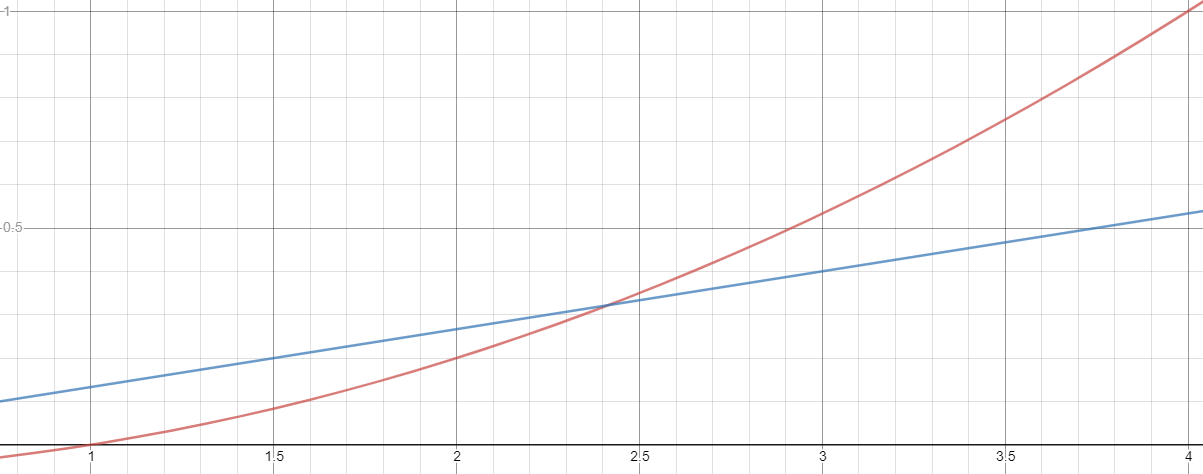
\includegraphics[width=5in]{cdf.png}
\end{figure}

The expectation for a continuous random variable is given as,
\begin{align*}
    \int_1^4 R \times \text{pdf} dR
    &= \int_1^4 R \times \frac{2R}{15} dR \\
    &= \int_1^4 \frac{2R^2}{15} dR \\
    &= \frac{2}{45} [64-1] \\
    &= \frac{126}{45} \\
    &= 2.8
\end{align*}

\section{PGF}
The properties of a probability generating function are as follows,
\begin{align*}
    \text{Expectation} &= G'(1) &= \frac{2}{3} \\
    \text{Variance} &= G''(1) + G'(1) - (G'(1))^2 &= \frac{5}{9} \\
    & G''(1) + \frac{2}{3} - \frac{4}{9} &= \frac{5}{9} \\
    & G''(1) &= \frac{1}{3} \\
\end{align*}

We know try find the generating function.
\begin{align*}
    G(z) &= E(z^x) \\
    &= \sum_{x=0}^\infty z^x P(X=x) \\
    &= z^0 P(X=0) + z^1 P(X=1) + z^2 P(X=2) \\
    G'(z) &= P(X=1) + 2z P(X=2) \\
    G''(z) &= 2P(X=2) \\
\end{align*}

We now use our derivatives to solve the pgf.
\begin{align*}
    G''(1) = 2P(X=2) &= \frac{1}{3} \\
    P(X=2) &= \frac{1}{6}
\end{align*}
\begin{align*}
    G'(1) = P(X=1) + 2P(X=2) &= \frac{2}{3} \\
    P(X=1) + \frac{1}{3} &= \frac{2}{3} \\
    P(X=1) &= \frac{1}{3} \\
\end{align*}

The remaining probability must be $P(X=0) = \frac{1}{2}$. Thus the pgf is
\begin{align*}
    G(z) &= z^0 P(X=0) + z^1 P(X=1) + z^2 P(X=2) \\
    &= \frac{1}{2} + z^1 \frac{1}{3} + z^2 \frac{1}{6} \\
\end{align*}

\begin{figure}[H]
    \centering
    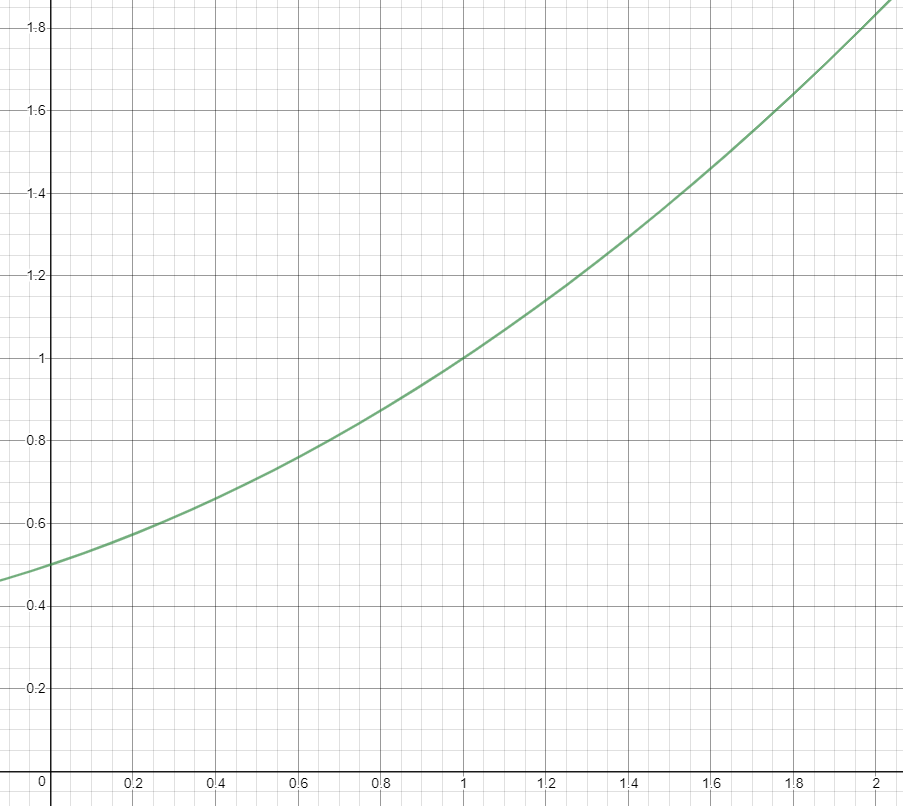
\includegraphics[width=5in]{pgf.png}
\end{figure}

\section{PDF}
\subsection{Find $c$}
A pdf has an integral the adds to one. Thus,
\begin{align*}
    \int_{-\infty}^\infty f(x) dx &= 1 \\
    \int_{2}^\infty \frac{c}{x^4} dx &= 1 \\
    \frac{-c}{3} \left[ \frac{1}{x^3} \right]_{x=2}^{x\to\infty} &= 1 \\
    \frac{-c}{3} \left[ 0 - \frac{1}{8} \right] &= 1 \\
    \frac{c}{24} &= 1 \\
    c &= 24 \\
\end{align*}

\subsection{Expectation}
We use the standard expectation and variance formulas
\begin{align*}
    \text{Expectation} &= \int_{-\infty}^{\infty} x f(x) dx \\
    &= \int_{2}^{\infty} x \frac{24}{x^4} dx \\
    &= 24 \int_{2}^{\infty} \frac{1}{x^3} dx \\
    &= -12 \left[ \frac{1}{x^2} \right]_{x=2}^{x\to\infty} \\
    &= -12 \left[ 0 - \frac{1}{4} \right] \\
    &= 3 \\
\end{align*}

\begin{align*}
    \text{Second moment} &= \int_{-\infty}^{\infty} x^2 f(x) dx \\
    &= \int_{2}^{\infty} x^2 \frac{24}{x^4} dx \\
    &= 24 \int_{2}^{\infty} \frac{1}{x^2} dx \\
    &= -24 \left[ \frac{1}{x} \right]_{x=2}^{x\to\infty} \\
    &= -24 \left[ 0 - \frac{1}{2} \right] \\
    &= 12 \\
\end{align*}

\begin{align*}
    \text{Variance} &= E(X^2) - (EX)^2 \\
    &= 12 - 3 \\
    &= 9 \\
\end{align*}

\subsection{Evaluate an expression}
\begin{align*}
    P(X > 4 | X > 3) &= \frac{P(X > 3 | X > 4)P(X > 4)}{P(X > 3)} \\
    &= \frac{P(X > 4)}{P(X > 3)} \\
    &= \frac{\text{cdf}(X > 4)}{\text{cdf}(X > 3)} \\
    &= \frac{\int_{4}^\infty f(x) dx}{\int_{3}^\infty f(x) dx} \\
    &= \frac{\left[ 0 - \frac{1}{64} \right]}{\left[ 0 - \frac{1}{27} \right]} \\
    &= \frac{27}{64} \\
    &= 0.421875 \\
\end{align*}

\section{Birthday}
I used the following code to simulate birthdays.
\verbatiminput{birthday.py}

It gave the following output in Python3
\begin{verbatim}
Expectation: 23.6113
\end{verbatim}

\end{document}
